\documentclass[11pt]{article}

\usepackage{amsmath,mathtools,siunitx,amssymb}
\usepackage[a4paper,left=1.5cm,right=1.5cm,top=2cm,bottom=2cm]{geometry}
\usepackage{float,subcaption,graphicx}
\usepackage{enumitem,pifont}
\renewcommand{\labelitemi}{\ding{228}}
\renewcommand{\labelitemii}{\ding{229}}
\renewcommand{\labelitemiii}{\ding{225}}
\setlist[itemize]{noitemsep}
\usepackage[dvipsnames]{xcolor}
\usepackage{color,hyperref}
\hypersetup{colorlinks=true}

\newcommand{\tVVt}{\frac{|\tilde{V}_{ij}|^2}{|V_{ij}|^2}}
\newcommand{\tVV}{\frac{|\tilde{V}_{ij}|}{|V_{ij}|}}

\begin{document}
{\Large\bfseries CKM Modification for paper draft}
\section{Basic Framework}
In the 2HDM, the Branching Ratio of a tree-level leptonic decay of a meson M can be written as
\begin{equation}
    \label{eq:brrh}
    \mathcal{B}r_{exp}[M\to l\nu_l] = \mathcal{B}r_{SM}[M\to l\nu_l]\times(1+r_H)^2.
\end{equation}
Here, $(1+r_H)^2$ describes the 2HDM correction factor, where for the meson M consisting of the up-type quark $q_u$ and down-type quark $q_d$,
\begin{equation}
    r_H = \left(\frac{m_{q_u}-m_{q_d}\tan^2\beta}{m_{q_u}+m_{q_d}}\right)\left(\frac{m_M}{m_{H^+}}\right)^2.
\end{equation}
This description of the 2HDM modification is convenient for working with leptonic decays, however when also considering semileptonic decays, $r_H$ can be broken down further into contributions to two Wilson coefficients for scalar operators defined as:
\begin{align}
    \label{eq:csr}
    \mathcal{O}_{SR} = -\frac{4G_F}{\sqrt{2}}V_{ub}(\bar{u}_Lb_R)(\bar{\mu}_R\nu_{\mu L}) &\to C_{SR} = \frac{m_u}{m_{H^+}^2} \\
    \label{eq:csl}
    \mathcal{O}_{SL} = -\frac{4G_F}{\sqrt{2}}V_{ub}(\bar{u}_Rb_L)(\bar{\mu}_L\nu_{\mu R}) &\to C_{SL} = \frac{m_b\tan^2\beta}{m_{H^+}^2} 
\end{align}
In Eq.\eqref{eq:brrh}, the CKM element $|V_{ij}|^2$ is included in $\mathcal{B}r_{SM}$, but if the 2HDM is realistic, then what we measure from experiment for the value of $|V_{ij}|^2$ from leptonic processes is really $|V_{ij}|^2\times(1+r_H)^2$, and there will be a similar factor for the measurement from semileptonic process.

It is still possible for the measured CKM elements to be correct in the 2HDM, in certain limits:
$r_H=0$ means that we are in the decoupling limit of the 2HDM, and we return to the SM theory being correct;
$r_H=-2$ means that we are in the fine-tuned solution of the 2HDM and what we measure as the SM CKM element is the correct value, although the 2HDM can still have non-negligible results elsewhere.
For $r_H\neq0,-2$, the true CKM element will be different from that measured in experiment and we cannot use the given SM values.
Therefore when testing if the 2HDM is correct, we must also assume that our values of CKM elements need modified.
Now for leptonic meson decays, we can rewrite Eq.\eqref{eq:brrh} as
\begin{equation}
    \mathcal{B}r_{exp} = \mathcal{B}r_{SM}\times\tVVt(1+r_H)^2,
\end{equation}
with $\tilde{V}_{ij}$ being the `real' CKM element value and $V_{ij}$ being the measured one in the SM.
This cancels the SM CKM value included in $\mathcal{B}r_{SM}$ and inputs the `real' one, if there is a difference in their value.

\section{Mapping Out the Modification}
The fraction $\tVV$ is then the modification factor that the measured CKM element must receive in the 2HDM to be the true CKM element. 
This factor for leptonic decays can be written as
\begin{align}
    \label{eq:modfac}
    |V_{ij}|^2 = |\tilde{V}_{ij}|^2(1+r_H)^2 \implies \frac{1}{(1+r_H)} = \tVV.
\end{align}
Using this form, and a similar structure for the semileptonic decays, the size of the modification factor $\tVV$ can be scanned across the 2HDM parameter space $(\tan\beta,m_{H^+})$ to test the significance of the factor for each $V_{ij}$ where the accepted values are commonly taken from leptonic and semileptonic tree-level decays. 
For each of the CKM elements in the first two rows of the CKM matrix, the modification factor was found to be $\sim1$ to a high precision across most of the parameter space considered. 
\begin{figure}[H]
    \centering
    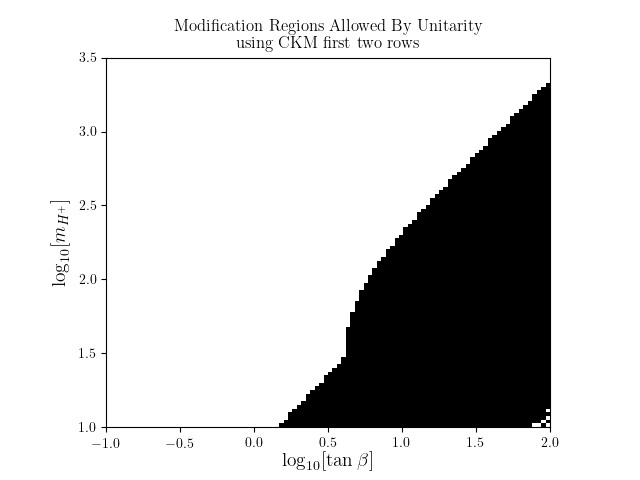
\includegraphics[width=0.32\textwidth]{heatmaps/mod.png}
    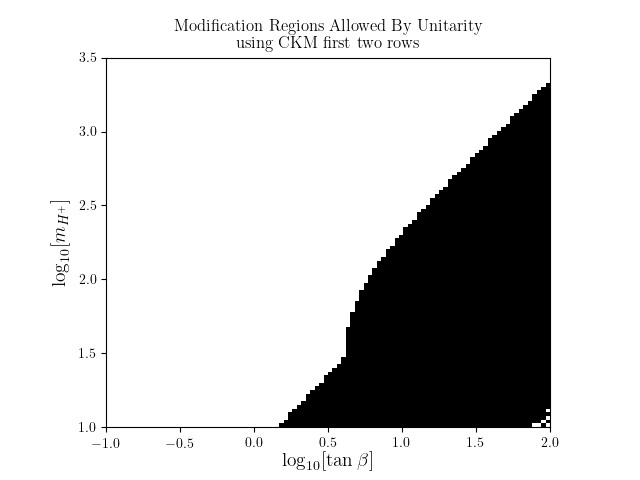
\includegraphics[width=0.32\textwidth]{heatmaps/mod.png}
    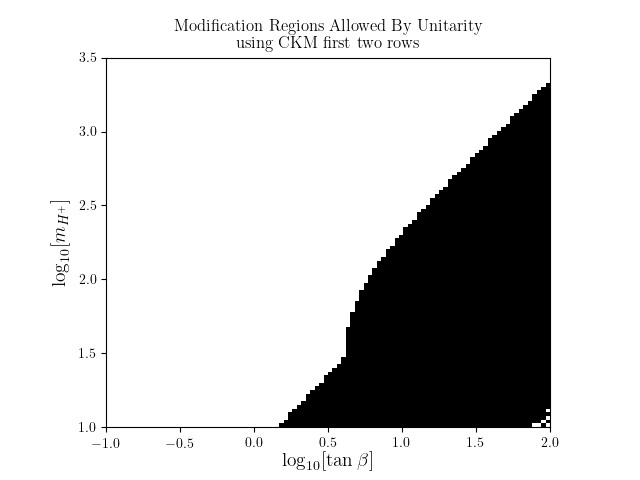
\includegraphics[width=0.32\textwidth]{heatmaps/mod.png}
    \caption{Heatmaps of the magnitude of the 2HDM modification factor for: $V_{ub}$ (left), $V_{us}$ (middle), $V_{cb}$ (right). \textbf{PLACEHOLDER IMAGE UNTIL UPDATED ONE IS FINISHED RUNNING}}
\end{figure}
The modification factor was found to significantly deviate from $1$ for high $\tan\beta$, low $m_{H^+}$, however this region is excluded by direct searches ($m_{H^+}\gtrsim160\,$GeV) and $B\to X_s\gamma$ in Section ref ($m_{H^+}\gtrsim890\,$GeV).
Therefore when considering tree-level processes involving quark currents of the first two CKM rows, it is appropriate to neglect the effects of a modification factor in the use of CKM elements in our calculations. 

In our consideration of the 2HDM for flavour observables in Section ref, however, we do not limit ourselves to these processes, so we use some of the CKM elements we can modify to construct the CKM matrix in the 2HDM. 
We use the standard phase convention and tree-level parameterisation where 
\begin{align}
    V_{us} &= \cos\theta_{13}\sin\theta_{12}, & |V_{ub}| &= |\sin\theta_{13}|, & V_{cb} &= \cos\theta_{13}\sin\theta_{23}, & \gamma = \delta.
\end{align}
The full CKM matrix can then be constructed from the four parameters $V_{us},|V_{ub}|,V_{cb},\gamma$, and so it is the 2HDM modification of these that must be considered. 
Considering the definition of $\gamma$,
\begin{equation}
    \gamma = \text{arg}\left(-\frac{V_{ud}V_{ub}^*}{V_{cd}V_{cb}^*}\right),
\end{equation}
it is expected that this will receive no 2HDM contribution as it deals with the complex phases of the CKM elements and not the magnitude which is modified in the 2HDM.
The three CKM elements averaged from leptonic and semileptonic decays will still be modified as discussed above, so there is possibility for the whole CKM matrix to be changed. 
From the above discussion of the modification of single CKM elements, the modification factor has negligible effect within regions that are not already excluded, so within these regions, none of the CKM elements calculated should gain significant contributions. 
As a test of this, a $2\sigma$ confidence scan was performed in the 2HDM parameter space checking where CKM matrix unitarity is violated.
\begin{figure}[H]
    \centering
    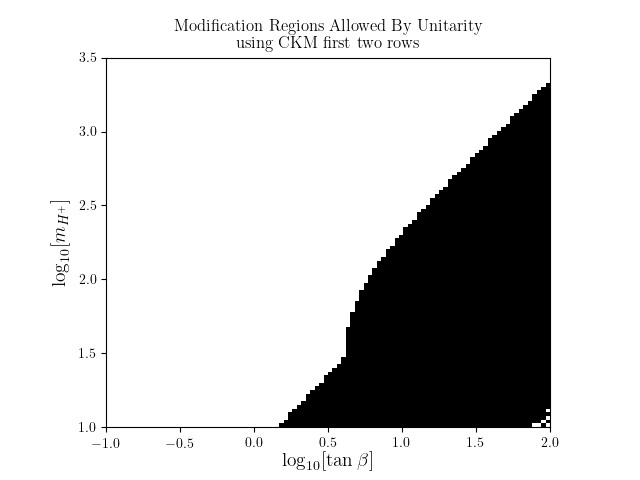
\includegraphics[width=0.45\textwidth]{heatmaps/mod.png}
    \caption{The black region represents areas where the CKM matrix unitarity is violated in the 2HDM as discussed above; the white is where unitarity is still possible within $2\sigma$. \\ \textbf{PLACEHOLDER IMAGE UNTIL UPDATED ONE IS FINISHED RUNNING}}
\end{figure}

\section{Conclusions}
From the scans of the magnitudes of the CKM elements and the unitarity tests, it becomes a reasonable assumption to neglect modification to the CKM elements in our fits in Section ref.
The validity of this assumption does not hold when considering low $m_{H^+}$, high $\tan\beta$ but this region is excluded by direct search limits and the radiative $B\to X_s\gamma$ decay. 
Therefore this assumption proves valid within regions not already excluded. 

Were the 2HDM proven to be physical, it could be the case that there is some small modification to CKM elements that although is not enough to impact results here, would need to be considered. 
This would be dependent on the specific values found for $m_{H^+}$ and $\tan\beta$ from experiment.

\end{document}












